\documentclass[times, utf8, zavrsni, numeric]{fer}
\usepackage{booktabs}
\usepackage{pdfpages}
\usepackage{comment}
\usepackage{float}
\usepackage{amsthm}
\usepackage{amsmath}
\usepackage{amssymb}

\newtheorem{theorem}{Teorem}
\newtheorem{definition}{Definicija}
\newtheorem{korolar}{Korolar}
\newtheorem{proposition}{Propozicija}


\begin{document}

\thesisnumber{851}

\title{Igre na grafovima}

\author{Filip Ćelepirović}

\maketitle


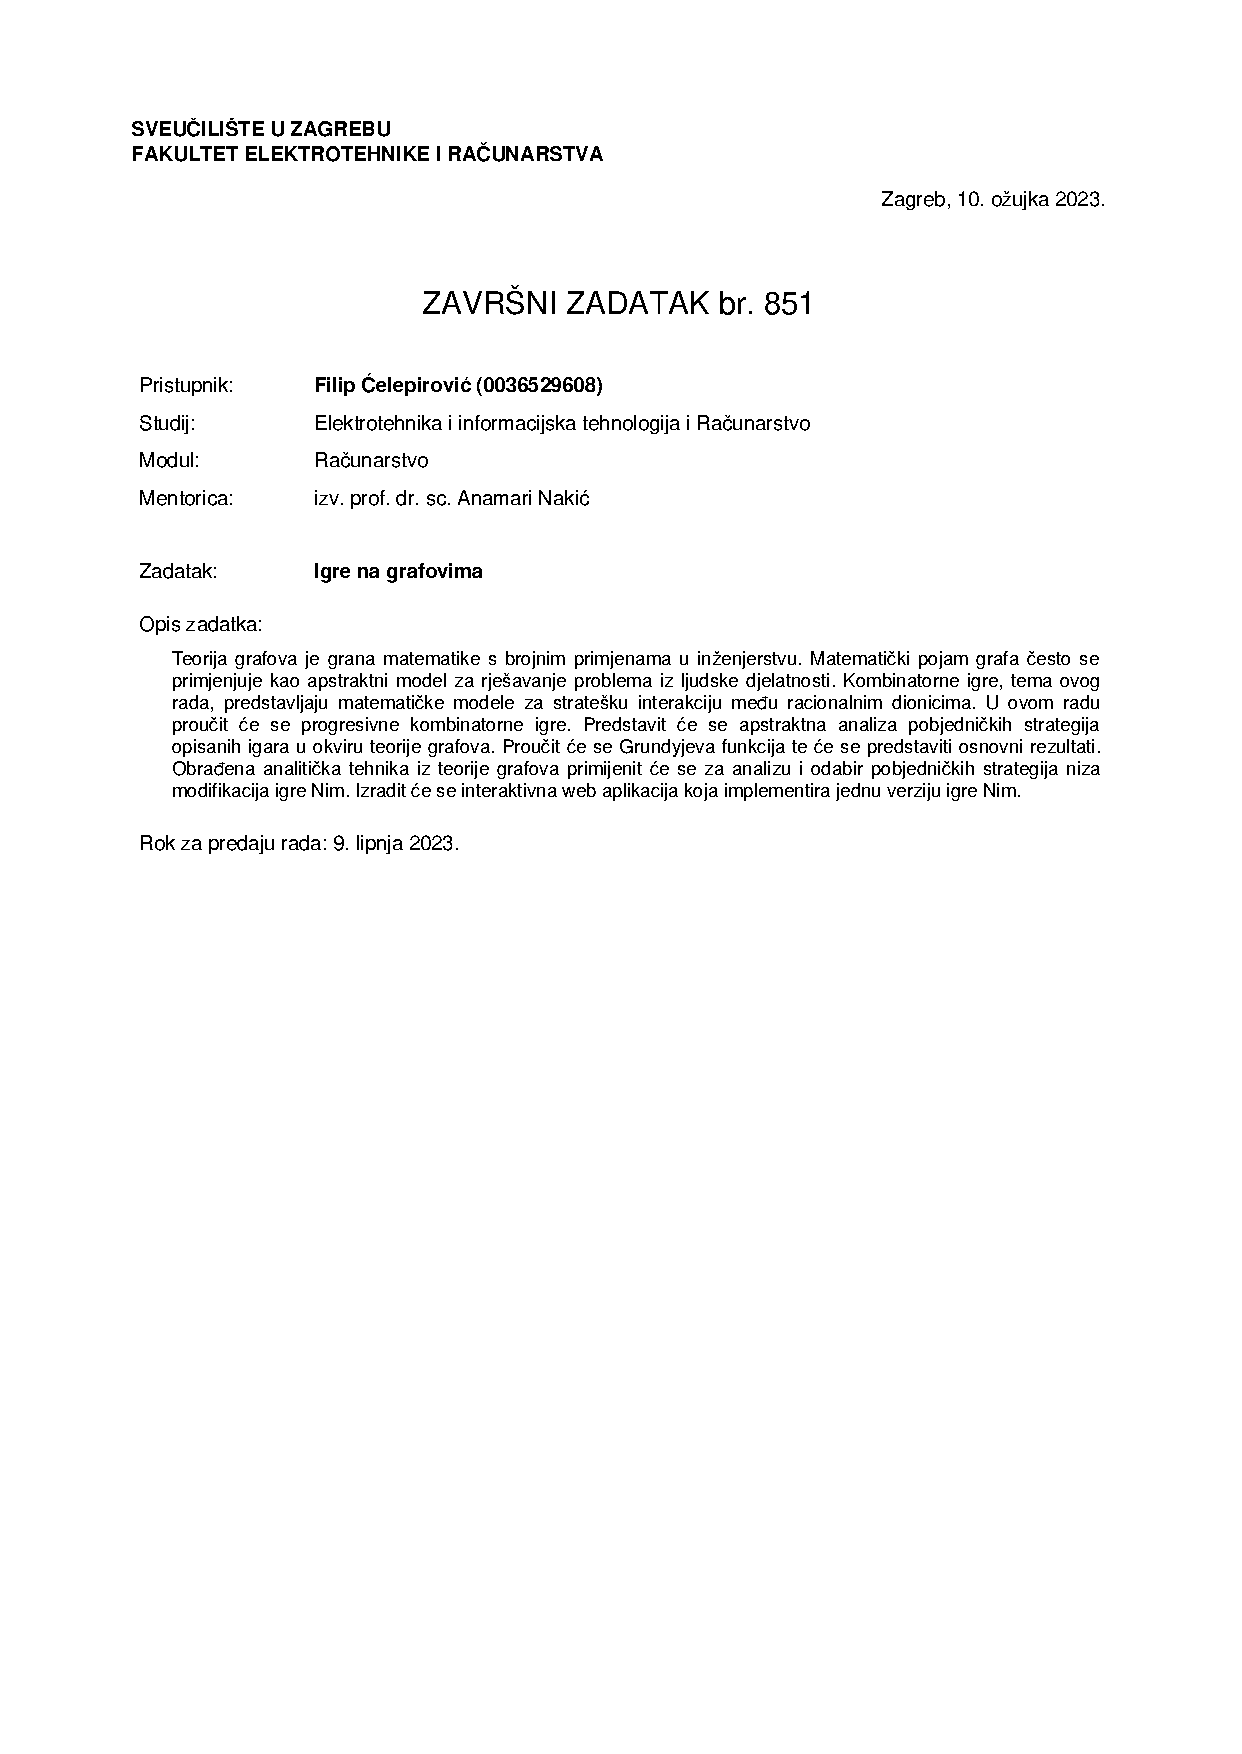
\includepdf[]{izvornik.pdf}

\zahvala{Posebna zahvala mojim roditeljima na podršci tijekom cijelog školovanja. Također, želim zahvaliti mentorici prof. Nakić na potpori i pomoći u izradi ovog završnog rada.}

\tableofcontents
\listoffigures
\listoftables



\chapter{Uvod}
Teorija grafova vrlo je važna grana matematike koja se primjenjuje u mnogim poljima znanosti, kao što su računalna znanost, inženjerstvo, ali i u društvenim znanostima. Koncept grafa je apstraktni model koji se koristi za rješavanje različitih problema u ljudskom djelovanju. S druge strane, kombinatorne igre predstavljaju matematičke modele za stratešku interakciju između racionalnih dionika.

Ovaj rad proučava progresivne kombinatorne igre i predstavlja apstraktnu analizu njihovih pobjedničkih strategija koristeći teoriju grafova. Konkretno, u fokusu je Grundyjeva funkcija, koja se koristi za određivanje ishoda kombinatornih igara.

Analiza pobjedničkih strategija ključna je jer pomaže u razumijevanju procesa donošenja odluka i pruža uvid u međusobnu stratešku komunikaciju. Korištenje teorije grafova u ovoj analizi omogućuje nam modeliranje složenih sustava i njihovu strukturiranu i detaljnu analizu.

Nadalje, primijenjena je razrađena analitička tehnika iz teorije grafova za analizu i odabir optimalnih pobjedničkih strategija za niz modifikacija igre Nim. Nim je klasična kombinatorna igra koja je opsežno proučavana u literaturi i ima brojne primjene u računalnim znanostima i inženjerstvu.

Kako bismo analizu kombinatornih igara učinili što pristupačnijom i kao rezultat cjelokupne teorijske analize, izrađena je interaktivna web aplikacija koja implementira jednu verziju igre Nim. To omogućuje korisnicima da eksperimentiraju s igrom i bolje usavrše razumijevanje koncepata igre o kojima se govori u ovom radu.

Sveukupno, cilj je ovog rada pružiti sveobuhvatnu analizu kombinatornih igara i njihovih pobjedničkih strategija korištenjem teorije grafova.


\chapter{Osnovni pojmovi}
 \section{Uvod i definicija}

Kombinatorne igre vrsta su igara u kojima se igrači bore za kontrolu nad skupom objekata, poput figura na šahovnici ili polja na ploči. Ove igre zovu se kombinatorne jer se igrači bore za kontrolu nad kombinacijom objekata i svojom strategijom igrači koriste svoje znanje i vještinu za kontrolu igre i ukupnu pobjedu.\newline

Za svaku kombinatornu igru vrijede sljedeći uvjeti\cite{garner2007combinatorialgametheory}:

\begin{itemize}
    \item Dva igrača: Kombinatorne igre igraju se između dva igrača, koji mogu biti označeni različitim bojama, znakovima ili samo kao prvi i drugi igrač. 
    \item Nema elemenata slučajnosti: U kombinatornim igrama, nema faktora slučajnosti koji bi utjecali na ishod igre. To znači da potezi koje igrači čine nisu određeni kockanjem, srećom ili nasumičnim događajima, već samo njihovom strategijom.
    \item Potpuna informacija: Svaki igrač u kombinatornoj igri ima potpuni uvid u sve informacije o trenutnom stanju igre. Nema skrivanja idućeg poteza, svaki igrač zna sve što je javno dostupno.
    \item Naizmjenična igra: Kombinatorne igre igraju se naizmjenično između dva igrača. Svaki igrač izvodi poteze jedan za drugim, izmjenjujući se dok igra ne završi.
    \item Postoji pobjednik: U kombinatornim igrama, jedan igrač uvijek mora pobijediti, a drugi izgubiti. Nema neodlučenog rezultata kao što je remi u šahu.
    \item Uvjet pobjede: Da bi igrač pobijedio, potrebno je doći do krajnje pozicije igre koja je unaprijed definirana. Ova krajnja pozicija može biti, na primjer, osvajanje protivničkog kralja u šahu ili postizanje zadane razine bodova u igri kao što je Go. 
\end{itemize}


Također, moramo uvesti još jedan pojam, a to je nepristrana igra\cite{2001winningwaysforyourmathematicalplays}.

\begin{definition}
Igra je nepristrana ako i samo ako oba igrača imaju iste mogućnosti poteza za svaku trenutnu poziciju u igri.
\end{definition}
 


U svim nepristranim kombinatornim igrama postoje dvije vrste pozicija: \textit{P-pozicije} (engl. previous) i \textit{N-pozicije} (engl. next). P-pozicije su pozicije u kojima prethodni igrač ima pobjedničku strategiju, a sukladno tome, N-pozicije su pozicije u kojima sljedeći igrač ima pobjedničku strategiju. Postupak za određivanje vrste pozicije kojoj pripada određena pozicija započinje identificiranjem završnih, terminalnih pozicija kao P-pozicija. Zatim se identificiraju pozicije koje vode do P-pozicija i označavaju se kao N-pozicije. Nakon toga, traže se pozicije iz kojih se dolazi samo do N-pozicija i takve pozicije se označavaju kao P-pozicije, a to se sve ponavlja dok se ne odrede i identificiraju sve moguće pozicije u igri kao P-pozicije ili N-pozicije.

Ova podjela na P-pozicije i N-pozicije korisna je pri razvoju pobjedničke strategije u igri jer je cilj svakog igrača dovesti igru u P-pozicije, a to su pobjedničke pozicije. Također, početna pozicija određuje koji igrač ima pobjedničku strategiju. U idućem poglavlju analizirat ćemo P-pozicije i N-pozicije na primjerima igre 21 i igre Nim. 



\section{Primjeri kombinatornih igara}

Postoje brojne popularne kombinatorne igre, a ovdje ćemo nabrojati samo neke od njih:

\subsection*{Igra oduzimanja}

Vjerojatno najjednostavniji mogući primjer jedne nepristrane kombinatorne igre je \textit{igra oduzimanja}. U igri oduzimanja dva igrača miču jedan, dva ili tri žetona sa hrpe koja se sastoji od 21 žetona. Gubitnik je onaj igrač koji ukloni zadnji žeton. Postoji mnogo mogućih varijacija ove igre, od broja dozvoljenih žetona koji se mogu ukloniti u jednom potezu, do ukupnog broja žetona na hrpi. U nastavku analize pokazat ćemo kako varijacije utječu na rezultat igre i strategiju igrača.



\subsection*{Nim}


Igra Nim također je jedna jednostavna igra za dva igrača u kojoj se, za razliku od igre oduzimanja, koristi više hrpa žetona. Svaka hrpa žetona može imati proizvoljan broj žetona, a broj hrpa može biti različit od igre do igre. Na početku igre, igrači se dogovaraju o broju hrpa i broju žetona u svakoj hrpi.

Tijekom igre, igrači naizmjence uzimaju žetone s ploče za igru. Svaki igrač mora uzeti žetone samo iz jedne hrpe, ali može uzeti bilo koji broj žetona iz te hrpe. Nakon što igrač uzme žetone, on ih uklanja s ploče za igru.

Cilj igre je ostati s barem jednim žetonom na ploči, tako da protivnik ne može uzeti zadnji žeton. Uzimanje zadnjeg žetona predstavlja gubitak igre, a pobjednik je onaj koji uspije natjerati protivnika da uzme zadnji žeton.

\begin{figure}[H]
\centering
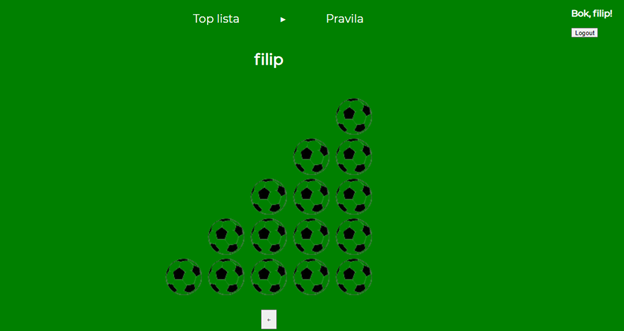
\includegraphics[width=14cm]{slike-program/Slika6.png}
\caption{Igra Nim.}
\label{}
\end{figure}


\subsection*{Hex}

Igra Hex igra je za dva igrača koja se igra na šesterokutnoj ploči koja se sastoji od šestokutnih polja. Jedan igrač igra s bijelim figurama, a drugi s crnim figurama. Igrači igraju naizmjenično, stavljajući svoje figure na polja ploče.

Cilj igre je stvoriti poveznicu između dvije suprotne strane šesterokuta koju čine igračeve figure. Bijeli igrač pokušava stvoriti poveznicu između suprotne bijele strane ploče, dok crni igrač pokušava stvoriti poveznicu između suprotne crne strane ploče. Pobjeđuje igrač koji prvi uspije stvoriti poveznicu od jedne do druge strane ploče.

Figure se mogu postavljati na bilo koje slobodno polje na ploči. Igrači nastoje blokirati protivnika i povezati svoje figure kako bi stvorili poveznicu. Igrači također pokušavaju onemogućiti stvaranje poveznice za protivnika.


\subsection*{Go}

Igra Go igra je za dva igrača koja se igra na ploči veličine 19x19 polja, ali može se igrati i na manjim pločama. Jedan igrač igra crnim figurama, dok drugi igrač igra bijelim figurama. Igrači igraju naizmjenično, stavljajući svoje figure na prazna polja ploče.

Cilj igre je osvojiti što više teritorija na ploči postavljanjem svojih figura na prazna polja i stvaranjem zatvorenih prostora oko tih figura. Figura se naziva kamenom, a igrači ih postavljaju na presjecišta linija koje čine ploču.

Kamenovi se mogu postavljati na bilo koje prazno polje, ali ne smiju se postavljati na polja koja su već okupirana od strane protivnika. Kada jedan igrač okruži prazna polja kamenovima, taj teritorij smatra se osvojenim.

Osim osvajanja teritorija, igrači također mogu zarobiti protivničke kamenove. Kamen se zarobi kada se okruži na sve strane praznim poljima ili poljima s kamenovima iste boje. Zarobljeni kamen se uklanja s ploče.

Igra Go je za razliku od ostalih navedenih igara vrlo složena i strateški izazovna igra u kojoj  igrači pokušavaju predvidjeti poteze protivnika i stvoriti najbolju strategiju za osvajanje teritorija.


\chapter{Analiza kombinatornih igara}
U ovom poglavlju prikazat ćemo analizu kombinatornih igara i matematičku teoriju koja se nalazi u pozadini. 


\section{Analiza igre oduzimanja}

Analizu igre oduzimanja započet ćemo od kraja prema početku. Ako je na hrpi ostao samo jedan, dva ili tri žetona igrač koji je idući na redu pobjeđuje uzimanjem svih preostalih žetona pa su zbog toga te pozicije N-pozicije. 

Sada pretpostavimo da je ostalo četiri žetona. Ako igrač koji miče sljedeći uzme jedan ili dva žetona, protivnik mu može uzvratiti na način da ostavi hrpu sa jednim ili dva žetona, čime on dolazi u poziciju da gubi u igri. Međutim, ako igrač koji miče sljedeći uzme sva tri, ostavlja jedan žeton na hrpi. Tada njegov protivnik mora uzeti preostali žeton, a igrač koji je bio na potezu prije njega pobjeđuje pa je pozicija s 4 žetona P-pozicija.

Ako je na hrpi 5, 6 ili 7 žetona, trenutni igrač može uzeti dovoljno žetona da dovede protivnika u stanje igre u P-poziciju s 4 žetona. To znači da ako igrač uzme x žetona, njegov protivnik će morati uzeti (4 - x) žetona, što će ga dovesti u poziciju s 4 žetona, gdje će izgubiti. Zbog toga su pozicije s 5, 6 ili 7 žetona na hrpi N-pozicije.

Kada se na hrpi nalazi 8 žetona, igrač koji je tada na potezu ne može ostaviti protivnika u P-poziciji s 4 žetona, što znači da je stanje igre s 8 žetona na hrpi klasificirano kao P-pozicija.

Slično kao u navedenim primjerima, možemo izvesti prikaz P i N pozicija za svako stanje igre pa tako dolazimo do prikaza svih P i N pozicija u igri oduzimanja.

\begin{comment}

\begin{table}[H]
\caption{Prikaz P-pozicija i N-pozicija u igri oduzimanja}
\label{tbl:igra21}
\centering
\begin{tabular}{|c|c|c|c|c|c|c|c|c|c|c|c|c|c|c|c|c|c|c|c|c|c|}
\hline
0 & 1 & 2 & 3 & 4 & 5 & 6 & 7 & 8 & 9 & 10 & 11 & 12 & 13 & 14 & 15 & 16 & 17 & 18 & 19 & 20 & 21 \\
\hline
P & N & N & N & P & N & N & N & P & N & N & N & P & N & N & N & P & N & N & N & P & N \\
\hline
\end{tabular}
\end{table}

\end{comment}

\begin{table}[H]
\caption{Prikaz P-pozicija i N-pozicija u igri oduzimanja (1-11)}
\label{tbl:igra21_1-11}
\centering
\begin{tabular}{|c|c|c|c|c|c|c|c|c|c|c|c|}
\hline
0 & 1 & 2 & 3 & 4 & 5 & 6 & 7 & 8 & 9 & 10 & 11 \\
\hline
P & N & N & N & P & N & N & N & P & N & N & N \\
\hline
\end{tabular}
\end{table}


\begin{table}[H]
\caption{Prikaz P-pozicija i N-pozicija u igri oduzimanja(12-21)}
\label{tbl:igra21_12-21}
\centering
\begin{tabular}{|c|c|c|c|c|c|c|c|c|c|c|c|c|c|c|c|c|c|c|c|c|c|}
\hline
12 & 13 & 14 & 15 & 16 & 17 & 18 & 19 & 20 & 21 \\
\hline
P & N & N & N & P & N & N & N & P & N \\
\hline
\end{tabular}
\end{table}

Kao zaključak ove analize, možemo vrlo jednostavno definirati ova dva pravila:

\begin{enumerate}
\item Pozicija s koje je moguće pomaknuti se na P-poziciju je N-pozicija.
\item Ako je trenutna pozicija ona s koje se ne može doći do P-pozicije (to jest, svi su mogući potezi na N-pozicijama) ili ako nema više mogućih poteza, onda je to P-pozicija. 
\end{enumerate}

Lako je zaključiti da je svaka pozicija s n žetona, gdje je n = 4k, P-pozicija, a sve ostale pozicije (n = 4k + 1, n = 4k + 2, n = 4k + 3) su N-pozicije. Logičan dokaz toga jest činjenica da postoji potez od svakog broja koji nije djeljiv s 4 do onog koji je djeljiv s 4 (uzimajući jedan žeton u poziciji 4k + 1, dva žetona u poziciji 4k + 2 ili tri žetona u poziciji 4k + 3). 

Kada oba igrača primjete da je jasno od početka tko će biti pobjednik i da nakon prvog poteza samo izmjenjuju poteze, gdje jedan od njih uzima bilo koji broj žetona, a drugi odgovara tako da uzme ostatak od 4 igra postaje nezanimljiva, zbog čega ćemo u daljnjoj analizi nadograditi ovu igru tako što ćemo odvojiti žetone na više hrpa u igri Nim.

Analiza obrnutog oblika ove igre (misère) nije nimalo zahtjevnija od klasičnog oblika. U misère formi prisiljava se protivnika da mu na kraju ostane jedan žeton u posljednjem potezu, umjesto nijednog. Stoga su P-pozicije n = 4k + 1, a N-pozicije n = 4k, n = 4k + 2 i n = 4k + 3, a igrač koji započinje prvi je gubitnik.



\section{Analiza igre Nim}

\subsection*{N, P pozicije u igri Nim}

Slično kao i u igri oduzimanja, pronalaženje najbolje strategije za pobjedu započinje od završne, terminalne pozicije. To je pozicija u kojoj nema više žetona na ploči za igru. Ova pozicija može se ostvariti samo iz pozicije s jednom hrpom na kojoj se nalazi bilo koji broj žetona pa je pozicija s jednom hrpom N-pozicija. 

Igra s dvije hrpe nije nimalo kompliciranija. Prvi igrač bira hoće li ukloniti jedan žeton sa lijeve hrpe, jedan žeton sa desne hrpe ili oba žetona s desne hrpe. Ako ukloni samo jedan žeton s desne hrpe na kojoj se nalaze dva žetona protivnik će morati ukloniti jedan od preostalih žetona pa će prvi igrač pobijediti. U suprotnom, ukloni li prvi igrač oba žetona ili žeton s lijeve hrpe omogućit će protivniku pobjedu.

\begin{figure}[H]
\centering
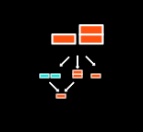
\includegraphics[]{slike-analiza/slika1.png}
\caption{Prikaz igre sa dvije hrpe.}
\label{}
\end{figure}


Sada razmotrimo malo zahtjevniji primjer, kada se u igri nalaze tri hrpe sa po jednim, dva i tri žetona. Pristup pronalaženju najboljih poteza ostaje isti. Uzmimo primjer najjednostavnije pozicije s tri hrpe, (1,1,1), kada se na svakoj od tri hrpe nalazi po jedan žeton. Vrlo je jednostavno zaključiti da u toj poziciji pobjeđuje prvi igrač jer ne postoji niti jedan potez koji bi omogućio drugom igraču da ostvari pobjedu. Zbog toga je pozicija (1,1,1) N-pozicija.

\begin{figure}[H]
\centering

\includegraphics[]{slike-analiza/slika2.png}
\caption{Prikaz pozicije s jednim žetonom na svakoj hrpi.}
\label{}
\end{figure}

Sljedeća pozicija koju bismo analizirali je pozicija (1,1,2). Postoje tri moguća poteza koje igrač može odigrati iz ove pozicije: (1,1), (1,2) ili (1,1,1). Pozicija (1,2) je također N-pozicija jer igrač koji je tada na potezu može odigrati potez koji će poziciju pretvoriti u (1,1), što je N-pozicija. Pozicija (1,1,1) je također N-pozicija, kao što smo već vidjeli. Ostaje nam razmotriti poziciju (1,1), koja predstavlja P-poziciju jer se radi o igri s dvije hrpe jednake veličine. S obzirom da postoji potez koji vodi iz pozicije (1,1,2) u P-poziciju (1,1), poziciju (1,1,2) također možemo proglasiti N-pozicijom.


\begin{figure}[H]
\centering
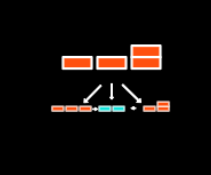
\includegraphics[]{slike-analiza/slika3.png}
\caption{Prikaz mogućih poteza iz pozicije (1,1,2).}
\label{}
\end{figure}

Sada ćemo analizirati poziciju (1,2,2). Svi mogući potezi iz ove pozicije su (1,1,2), (1,2) i (2,2). Pozicija (1,1,2) i pozicija (1,2) su N-pozicije, dok je pozicija (2,2) P-pozicija jer se radi o igri s dvije hrpe iste veličine. S obzirom da su svi mogući potezi iz pozicije (1,2,2) N-potezi, poziciju (1,2,2) također možemo proglasiti N-pozicijom.

Za analizu pozicije (1,2,3), postoji šest mogućih poteza. Pozicija (1,2) se identificira kao N-pozicija jer se može reducirati na (1,1) i (1,2) koje su obje N-pozicije. Pozicija (1,1,2) također je N-pozicija jer se može reducirati na (1,1) i (2), obje N-pozicije. 
Pozicija (1,2,2) je N-pozicija jer se može reducirati na (1,2) i (2), obje N-pozicije. Na isti način reduciramo pozicije (1,1,3) na (1,3) i (1,1,1), (1,3) na (1,2) i (1), (2,3) na (1,2) i (1,1).
 
Kada se sve pozicije analiziraju, može se napraviti stablo svih mogućih pozicija, koje pokazuje da se oba gore navedena pravila mogu primjeniti na igru Nim s tri hrpe: svaka P-pozicija ima samo djecu pozicije koje su N-pozicije, a svaka N-pozicija ima barem jedno dijete koje je P-pozicija. Na slici je svaka P-pozicija prikazana plavom bojom, a N-pozicija crvenom bojom.

\begin{figure}[H]
\centering
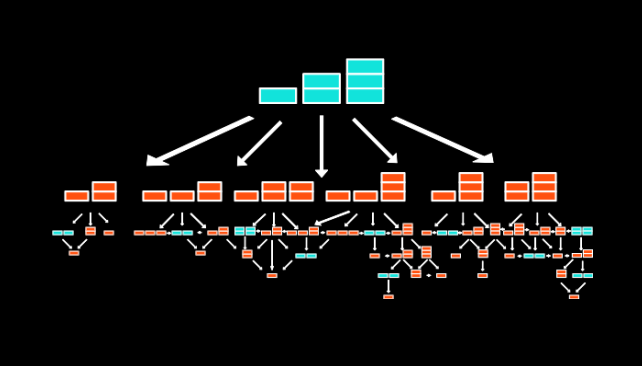
\includegraphics[]{slike-analiza/slika4.png}
\caption{Stablo svih mogućih pozicija u igri Nim s tri hrpe.}
\label{}
\end{figure}

Ako se ova analiza proširi na igru s više hrpa, proces pronalaženja P i N-pozicija postaje složeniji, ali osnovni principi ostaju nepromjenjeni. 



\subsection*{Nim vrijednost}

Svaku P i N-poziciju u igri Nim moguće je dobiti analizom u prethodnom poglavlju, no postavlja se pitanje praktičnosti analize igara s više hrpa, a samim time i većim veličinama hrpa. Zbog toga moramo uvesti bolje načine analize pozicija u igri Nim.

Jedan od novih i boljih načina analiza pozicija u igri Nim predstavili su matematičari Roland P. Sprague i Patrick M. Grundy.\cite{2008gametheoryferguson} Oni koriste binarne brojeve za opisivanje svakog stanja igre Nim, pri čemu se dekadski broj žetona na svakoj hrpi prebacuje u binarni oblik. Ukupna vrijednost pozicije nije samo vrijednost jedne hrpe, nego zbroj svih binarnih vrijednosti.

Definicija Nim zbrajanja glasi:
\begin{definition}
(x\textsubscript{n} x\textsubscript{n-1} $\dots$ x\textsubscript{1} x\textsubscript{0}) $\oplus$ (y\textsubscript{n} y\textsubscript{n-1} $\dots$ y\textsubscript{1} y\textsubscript{0}) = (z\textsubscript{n} z\textsubscript{n-1} $\dots$ z\textsubscript{1} z\textsubscript{0}), gdje je svaki z = (x + y) mod 2.
\end{definition}

Pomoću ove definicije možemo za svaku poziciju odrediti njezin Nim zbroj. No kako odrediti je li ta pozicija P-pozicija ili N-pozicija? Uzmimo ponovno za primjer igru Nim sa tri hrpe iz gornjeg primjera. Pretvorbom dekadske vrijednosti broja žetona na svakoj hrpi u binarni oblik dobivamo vrijednosti 1, 10 i 11.
Nim zbroj tih binarnih vrijednosti daje rezultat 0.

\begin{center}
1 = (\texttt{1})\textsubscript{2}\newline
2 = (\texttt{10})\textsubscript{2}\newline
3 = (\texttt{11})\textsubscript{2}\newline
\rule{2cm}{0.1pt}\newline
$\oplus$ = (\texttt{00})\textsubscript{2}\newline
\end{center}

Iz gornjeg primjera već znamo da je ta pozicija P-pozicija. Uzmimo sada kao primjer poziciju (1,2,2), za koju već znamo da je N-pozicija. Pretvorbom dekadskih vrijednosti u binarni oblik i Nim zbrajanjem dobivamo vrijednost 100.

\begin{center}
1 = (\texttt{1})\textsubscript{2}\newline
2 = (\texttt{10})\textsubscript{2}\newline
2 = (\texttt{10})\textsubscript{2}\newline
\rule{2cm}{0.1pt}\newline
$\oplus$ = (\texttt{01})\textsubscript{2}\newline
\end{center}

Na temelju navedenih primjera možemo zaključiti da su sve P-pozicije u igri Nim vrijednosti jednake 0, dok su sve N-pozicije u igri Nim vrijednosti različite od 0. To se može izraziti kroz sljedeći korolar.

\begin{korolar}\cite{tucker2002appliedcombinatorics}
Pozicija (x\textsubscript{1}, $\dots$, x\textsubscript{n}), n $\in$ N  je P-pozicija ako i samo ako
x\textsubscript{1} $\oplus$ $\dots$ $\oplus$ x\textsubscript{n} = 0
\end{korolar}

Funkcionalnosti ove dvije obrađene metode mogu se činiti sličnima, no analiza Nim vrijednosti ima veliki utjecaj tijekom igranja igre jer pruža brzu i jednostavnu metodu pronalaženja najboljeg poteza iz bilo koje pozicije u igri. Dok N-pozicije i P-pozicije pokazuju samo karakter trenutne pozicije bez metode određivanja kako odabrati najbolji mogući potez, pomoću Nim vrijednosti lako se može odrediti najbolja opcija za kretanje kroz igru.

Na primjer, zamislimo igru Nim sa tri hrpe koja ima više od tri žetona na svakoj hrpi. Uzmimo za primjer da su količine žetona na svakoj hrpi 25, 21 i 10. Pomoću N-pozicija i P-pozicija teško ćemo odrediti koji potez odigrati, no pomoću Nim vrijednosti to možemo vrlo lako učiniti. Pretvorbom u binarni oblik dobivamo vrijednosti 11001, 10101 i 1010, a Nim zbrajanjem dobivamo vrijednost 6, što je N-pozicija.

\begin{center}
25 = (\texttt{11001})\textsubscript{2}\newline
21 = (\texttt{10101})\textsubscript{2}\newline
10 = (\texttt{1010})\textsubscript{2}\newline
\rule{2cm}{0.1pt}\newline
$\oplus$ = (\texttt{100})\textsubscript{2}\newline
\end{center}

Najbolji izbor za igrača na potezu bi trebao biti svaki potez koji ima vrijednost Nim zbroja 0, što može lako napraviti ako pogleda zapis zbroja. Na primjer može uzeti dva žetona sa hrpe koja ima 21 žeton, što odmah mijenja Nim vrijednost u 0. Taj potez ostavlja protivnika u gubitničkoj poziciji i omogućava prvom igraču da dođe do pobjedničke pozicije.

\begin{center}
25 = (\texttt{11001})\textsubscript{2}\newline
19 = (\texttt{10011})\textsubscript{2}\newline
10 = (\texttt{1010})\textsubscript{2}\newline
\rule{2cm}{0.1pt}\newline
$\oplus$ = (\texttt{000})\textsubscript{2}\newline
\end{center}


\subsection*{Sprague-Grundyjeva funkcija}

Općenitiji način za analizu nepristrane igre je korištenje Sprague-Grundyjeve funkcije (S-G funkcija)\cite{1939mathematicsandgames} \cite{1973ubermathematischekampfspiele}. Prvo moramo upotrijebiti neke nove zapise koji općenito opisuju nepristrane igre kako bi se kasnije mogla definirati sama S-G funkcija. Ovaj novi zapis bit će predstavljen parom (X, F), gdje X označava sve pozicije u igri, a F je funkcija koja definira sve moguće pozicije x $\in$ X. Zbog činjenice da se svi potezi uvijek izvode iz jedne pozicije igre na skup pozicija, funkcija F nam daje podskup F(x) od X na svaku poziciju x $\in$ X. Drugim riječima, ova funkcija dodjeljuje sve dostupne pozicije za bilo koju odabranu poziciju u igri.

Formalna definicija Sprague-Grundyjeve funkcije slijedi u nastavku:

\begin{definition}\cite{2008gametheoryferguson}
    Sprague-Grundyjeva funkcija grafa (X, F) je funkcija g, definirana na skupu X, koja uzima nenegativne cjelobrojne vrijednosti, pri čemu vrijedi:

\begin{center}
    g(x) = min (n $\geq$ 0 : n $\neq$ g(y), y $in$ F(x))
\end{center}

\end{definition}

Sama definicija na prvi pogled izgleda poprilično zbunjujuća zbog korištenja rekurzije u definiciji. Međutim, algoritam postaje vrlo jednostavan za razumijevanje i primjenu kada se počne graditi od završne, terminalne pozicije. Sve terminalne pozicije imaju vrijednost 0, a skup F(x) je prazan. Vrijednost g od terminalnog položaja tada se dodjeljuje kao broj jednak minimalnoj vrijednosti skupa n $\in$ \{0, 1, 2...\}, što je 0. Uzimajući u obzir poziciju čiji je jedini sljedbenik terminalna pozicija, vrijednost funkcije postaje g(x) = 1.

Iz ovih uvjeta slijedi da je pozicija x P-pozicija ako je vrijednost Sprague-Grundyjeve funkcije 0, inače su sve ostale pozicije N-pozicije:

\begin{itemize}
    \item Ako je x terminalna pozicija, tada je g(x) = 0.
    \item Za poziciju x za koju je g(x) = 0, svi su sljedbenici y od x takvi da je g(y) $\neq$ 0.
    \item Za poziciju x za koju je g(x) $\neq$ 0, postoji barem jedan sljedbenik y za koji je g(y) = 0.
\end{itemize}

Iz tih uvjeta možemo izvesti iduću propoziciju:

\begin{proposition}
Ako je vrijednost funkcije g(x) jednaka 0 za određeni vrh x $\in$ X, tada se vrh x označava kao P-vrh na grafu.
\end{proposition}

Iz tih uvjeta lako možemo vidjeti da postoji sličnost u funkcionalnosti između analize pomoću S-G funkcije i analize P-pozicija i N-pozicija. Procjena prema N-pozicijama i P-pozicijama označava sva stanja koja mogu dosegnuti P-poziciju iz N-pozicije, dok S-G funkcija svemu tome dodjeljuje broj različit od 0. S druge strane, P-pozicija je definirana kao ona čiji su jedini sljedbenici N-pozicije, što se izražava S-G vrijednošću 0 i kao ona pozicija sa sljedbenicima S-G vrijednosti različitih od 0.




Kako bismo analizu kombinatornih igara učinili što pristupačnijom i kao rezultat cjelokupne teorijske analize, u idućim poglavljima analizirat ćemo izrađenu interaktivnu web aplikaciju koja implementira jednu verziju igre Nim. To će omogućiti korisnicima da eksperimentiraju s igrom i bolje usavrše razumijevanje koncepata igre o kojima se govori u ovom radu.

\chapter{Tehničke značajke razvijene aplikacije}
\section{Struktura aplikacije}

Ova aplikacija napravljena je pomoću HTML-a, CSS-a i JavaScript-a, a sastoji se od sljedećih dijelova: jedne HTML datoteke, jedne CSS datoteke, dvije JavaScript datoteke, jedne json datoteke i jedne slike koja prikazuje lopticu na ploči za igru.  Za izradu sučelja korišten je HTML u datoteci index.html, a za stil korisničkog sučelja korišten je CSS u datoteci nim.css. Glavna logika programa napisana je pomoću jezika JavaScript, u datotekama game.js i index.js. Baza podataka je datoteka users.json u kojoj su pohranjeni podaci o korisnicima i o njihovim igrama.

\begin{figure}[H]
\centering
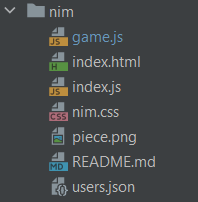
\includegraphics[]{slike-kod/Slika1.png}
\caption{Prikaz strukture koda aplikacije.}
\label{}
\end{figure}

Datoteka index.js sastoji se od tri funkcije: processPostRequest(), checkCredentials() i createServer(), koje služe za provjeru korisničkih podataka, obradu POST zahtjeva i kreiranje servera za pokretanje aplikacije.

Datoteka game.js prikazuje cjelokupnu logiku igre, a sastoji se od 15 funkcija gdje svaka funkcija ima svoju svrhu u samom programu. Funkcije koje se koriste u ovoj datoteci su:


\begin{itemize} 
\item showFrontPage() – prikaz početne stranice
\item showGameForm() -  prikaz stranice s postavkama igre
\item showRanks() – prikaz top liste najboljih igrača
\item showRules() – prikaz pravila igre
\item showGameDiv() – prikaz stranice sa igrom 
\item resetGameDiv() – uklanja stranicu s igrom
\item playGame() – inicijalizacija nove igre
\item restartGame() – ponovno pokretanje nove igre
\item login() – prijava korisnika u svoj profil
\item logout() – izlazak korisnika iz svog profila
\item leaveGame() – izlazak iz igre
\item Board() – prikaz ploče za igru
\item NimGame() – stvaranje nove igre
\item Piece() – stvaranje loptice na ploči za igru
\item PC() – određivanje poteza računala
\end{itemize}



\section{Funkcionalnosti aplikacije}



Funkcija checkCredentials() kao parametre prima korisničko ime i lozinku korisnika. Na početku pomoću funkcije createHash kreira hash lozinke korisnika. Ako to korisničko ime ne postoji u datoteci users.json, onda ga zajedno s tim hashom ubacuje u datoteku users.json, inače javlja grešku da je upisana lozinka pogrešna.  

Funkcija processPostRequest() kao parametre prima varijable zahtjeva i odgovora. Ona obrađuje POST zahtjeve ovisno o rezultatu poziva funkcije checkCredentials(). Ako je rezultat poziva funkcije jednak 2, vraća status 500, što označava grešku, a ako je rezultat poziva jednak 1 vraća status 400 s porukom da je korisnik registriran sa drugom lozinkom. U protivnom nema greške i vraća status 200. Na kraju datoteke pomoću funkcije createServer kreira se server na linku https://nim-projekt.onrender.com pomoću kojega se pokreće cijeli program.


\begin{figure}[H]
\centering
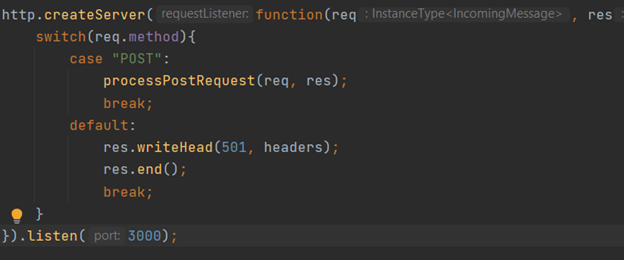
\includegraphics[width=14cm]{slike-kod/Slika2.png}
\caption{Prikaz koda funkcije createServer().}
\label{}
\end{figure}






Na početku datoteke game.js definiraju se sve varijable potrebne za pisanje programskog koda datoteke. Funkcija showFrontPage() prikazuje početnu stranicu i miče sve ostale elemente. Funkcija showGameForm() također miče sve ostale elemente, ali i ako igra još traje prikazuje ploču za igru i loptice. Također miče i formu u kojoj korisnik upisuje postavke igre. Ako korisnik nije ulogiran prikazuje formu za logiranje, a u suprotnom prikazuje formu za prikaz postavki igre. Ako upisana lozinka nije valjana prikazuje upozorenje o pogrešnoj lozinki, a isto to čini i za krivi upis veličine stupaca za igru.


\begin{figure}[H]
\centering
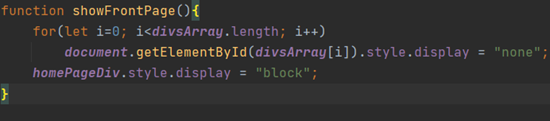
\includegraphics[width=14cm]{slike-kod/Slika3.png}
\caption{Prikaz koda funkcije showFrontPage().}
\label{}
\end{figure}

Funkcija showRanks() prikazuje top listu najboljih igrača. U tablici top lista nalaze se: korisničko ime igrača, ukupan broj njegovih igara, broj pobjeda, broj poraza i omjer njegovih pobjeda i poraza, a svi ti podaci upisuju se u users.json datoteku pomoću koje se ti podaci prikazuju korisniku. Tablica je sortirana prema omjeru pobjeda i poraza tako što je igrač sa najboljim omjerom na vrhu tablice. Funkcija showRules() prikazuje pravila igre nakon što korisnik klikne gumb za prikaz pravila igre, a s druge strane funkcije showGameDiv() i resetGameDiv() prikazuju i miču ploču s lopticama. 


\begin{figure}[H]
\centering
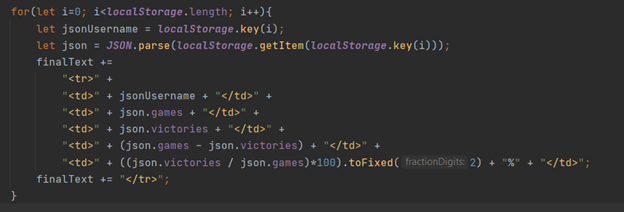
\includegraphics[width=14cm]{slike-kod/Slika4.png}
\caption{Prikaz tablice top lista iz funkcije showRanks().}
\label{}
\end{figure}


\begin{figure}[H]
\centering

\includegraphics[width=14cm]{slike-kod/Slika5.png}
\caption{Prikaz koda funkcija showRules(), showGameDiv() i resetGameDiv().}
\label{}
\end{figure}





Funkcija playGame() pomoću odabranih vrijednosti korisnika o veličini polja i igraču s prvim potezom inicijalizira novu igru, a prije toga provjerava je li upisana vrijednost veličine polja ispravna. Funkcija restartGame() samo ponovno poziva prethodno navedenu funkciju. Pomoću funkcije login() POST zahtjevom šalje se korisničko ime i lozinka igrača u datoteku users.json gdje se vodi evidencija o svim njegovim igrama, što se prikazuje u tablici igrača. Također, korisničko ime prikazuje se u gornjem desnom dijelu ekrana kako bi igrač mogao znati da je ulogiran u aplikaciju. Ako se igrač odluči izaći iz profila dok traje igra dobiva upozorenje da se to ne dozvoljava dok igra još traje, nego mu se to dozvoljava tek kada već započeta igra završi pa se prikazuje početna stranica. Također, kada igrač odluči izaći iz igre, ali ostati u svom profilu prikazuje mu se poruka o porazu i nudi se pokretanje nove igre. 



\begin{figure}[H]
\centering
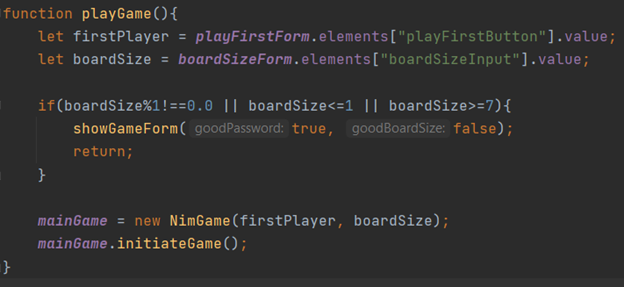
\includegraphics[width=14cm]{slike-kod/Slika6.png}
\caption{Prikaz koda funkcije playGame().}
\label{}
\end{figure}


\begin{figure}[H]
\centering

\includegraphics[width=14cm]{slike-kod/Slika7.png}
\caption{Prikaz koda funkcije login().}
\label{}
\end{figure}

\begin{figure}[H]
\centering

\includegraphics[width=14cm]{slike-kod/Slika8.png}
\caption{Prikaz koda funkcije logout().}
\label{}
\end{figure}


Ploča za igru izgrađena je od loptica koje su poredane uzlazno po stupcima tako što je u prvom stupcu jedna loptica, a svakim stupcem broj loptica se povećava za jednu, sve dok ne dođe do maksimalne razine koju je odredio korisnik u svojim početnim postavkama igre. Funkcija NimGame() inicijalizira novu igru tako što postavlja prvog igrača na potezu i kreira novu ploču za igru. Također, postavlja i poruku koji je igrač trenutno na potezu, koja se izmjenjuje svakim potezom, te oznaku da je igra u tijeku kako igrač ne bi mogao izaći iz svog profila tijekom igre.


\begin{figure}[H]
\centering
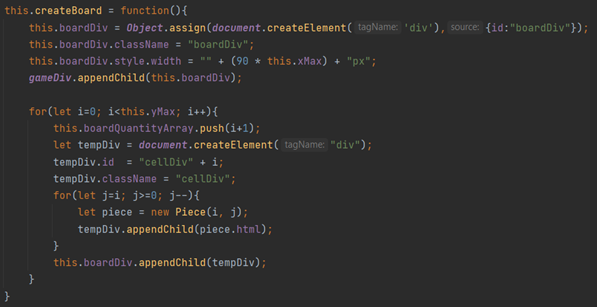
\includegraphics[width=14cm]{slike-kod/Slika9.png}
\caption{Prikaz koda za stvaranje ploče za igru.}
\label{}
\end{figure}


\begin{figure}[H]
\centering
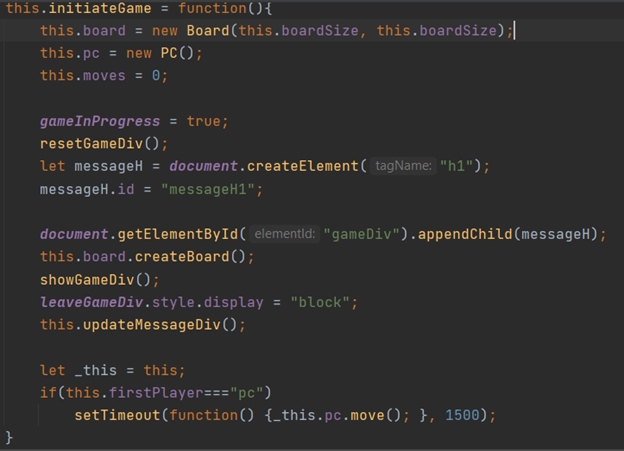
\includegraphics[width=14cm]{slike-kod/Slika10.png}
\caption{Prikaz koda za inicijalizaciju nove igre.}
\label{}
\end{figure}


 Klikom na lopticu ona se miče iz igre, a ako je to zadnja loptica na ploči, označava se kraj igre sa odgovarajućom porukom o pobjedniku, inače se provjerava koji je igrač bio na potezu i dozvoljava se drugom igraču da je na redu. Kada je igra gotova, u datoteku users.json igraču se dodaje nova igra i upisuje se je li pobijedio ili izgubio igru pa se sukladno tome računa i novi omjer pobjeda u igri. Korisnik tada može odlučiti igrati s istim ili drugačijim postavkama, a može i izaći iz profila i prestati igrati. Odlukom o izlasku iz igre dok igra traje također se u datoteku users.json dodaje nova igra i upisuje se da je korisnik poražen.

 


Glavni algoritam ovog programa je određivanje kakav će potez odigrati računalo i koje će loptice i u kojem stupcu ukloniti. Naime, u igri Nim s dva igrača, ako imamo n stupaca loptica (gdje se može ukloniti bilo koji broj loptica iz jednog stupca u jednom potezu) gubitničke su pozicije one u kojima je xor veličine stupca nije jednak 0. Zbog toga, računalo uvijek bira poteze u kojima (ako je to moguće na temelju korisnikovih poteza) xor veličine stupca nije 0 kako bi natjeralo korisnika da izgubi u igri.


\begin{figure}[H]
\centering
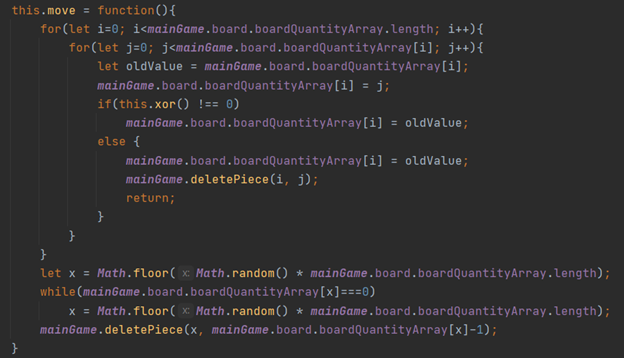
\includegraphics[width=14cm]{slike-kod/Slika11.png}
\caption{Prikaz određivanja novog poteza računala.}
\label{}
\end{figure}

\begin{figure}[H]
\centering
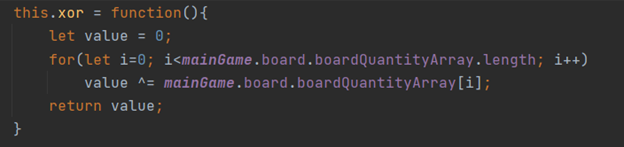
\includegraphics[width=14cm]{slike-kod/Slika12.png}
\caption{Prikaz funkcije xor().}
\label{}
\end{figure}





Pomoću funkcije Piece() stvara se nova loptica na ploči za igru. Kada je korisnik prešao mišem preko određenog broj loptica pomoću funkcije onmouseover označene loptice postaju bijele kako bi korisnik znao koje bi loptice uklonio eventualnim potezom. S druge strane, ako korisnik odustane od poteza, boja loptica ponovno postaje kakva je bila na početku bez uklanjanja. Tek klikom na lopticu korisnik uklanja loptice iz igre i čini svoj potez u igri, a loptice se tada brišu iz igre.


\begin{figure}[H]
\centering
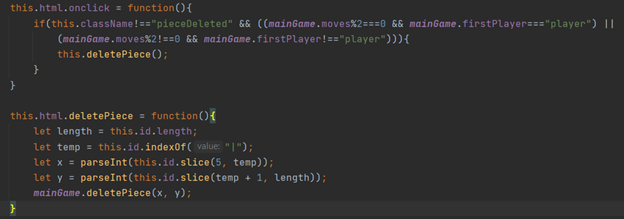
\includegraphics[width=14cm]{slike-kod/Slika13.png}
\caption{Prikaz funkcije za uklanjanje loptice iz igre.}
\label{}
\end{figure}

\chapter{Upute za korištenje razvijene aplikacije}
\input{Upute_za_korištenje_razvijene_aplikacije}

\chapter{Zaključak}
U ovom radu detaljno je proučena teorija i analiza kombinatornih igara. Teorija pruža alate i koncepte koji omogućuju modeliranje i analizu strateške interakcije u igrama. Kroz primjenu Grundyjeve funkcije, koja se temelji na teoriji grafova, možemo odrediti pobjedničke strategije u kombinatornim igrama.

Naglasak u izradi ovog rada je na progresivnim kombinatornim igrama, s posebnim fokusom na analizi niza modifikacija igre Nim. Primjena analitičke tehnike iz teorije grafova omogućila je dublje razumijevanje strukture i dinamike igre i identifikaciju optimalnih strategija za postizanje pobjede.

Uz teorijsku analizu, razvijena je i interaktivna web aplikacija koja implementira jednu verziju igre Nim. Ova aplikacija omogućuje korisnicima da igraju igru i istraže različite scenarije i strategije. 

S druge strane, kroz matematičke formalizme i analitičke tehnike, možemo bolje razumjeti kompleksne igre i identificirati optimalne strategije. Ovi rezultati imaju široku primjenu u područjima kao što su računalna znanost, matematika, inženjerstvo i društvene znanosti.

U zaključku, ovaj rad pruža sveobuhvatnu analizu kombinatornih igara. Njegovi rezultati i primjena Grundyjeve funkcije ukazuju na mogućnosti optimizacije strategija u igri Nim i sličnim situacijama.




\bibliography{literatura.bib}
\bibliographystyle{fer}

\begin{sazetak}

Ovaj rad proučava progresivne kombinatorne igre i predstavlja osnove analize pobjedničkih strategija. Primjenom Grundyjeve funkcije istražuju se osnovni rezultati i tehnike za odabir pobjedničkih strategija u nizu modifikacija igre Nim. Također, izrađena je interaktivna web aplikacija koja implementira jednu verziju igre Nim. Rezultati potvrđuju važnost matematičkog pristupa u analizi kombinatornih igara i njenu primjenjivost u inženjerskim područjima. 

\kljucnerijeci{teorija grafova, kombinatorne igre, pobjedničke strategije, Grundyjeva funkcija, igra Nim, web aplikacija}

\end{sazetak}


\engtitle{Graph games}

\begin{abstract}

This thesis examines progressive combinatorial games and presents the fundamentals of analyzing winning strategies. Through the application of Grundy's function, basic results and techniques for selecting winning strategies in a series of modifications of the game Nim are explored. Additionally, an interactive web application has been developed to implement one version of the game Nim. The results confirm the importance of a mathematical approach in the analysis of combinatorial games and its applicability in engineering fields.

\keywords{graph theory, combinatorial games, winning strategies, Grundy function, Nim game, web application}

\end{abstract}


\end{document}